\documentclass{standalone}
\usepackage{tikz}
\usetikzlibrary{arrows}
\usetikzlibrary{fadings}

\usepackage{stix}

\def\one{1}
\def\phi{\one*1.618}
\def\minr{sqrt(2*\one)}
\def\majr{\minr*\phi}
\def\maxr{\one+\phi}

\begin{document}

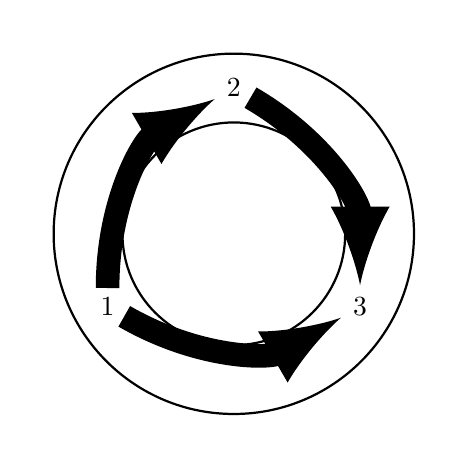
\begin{tikzpicture}[->,>=stealth',shorten >=1pt,auto,node distance=3cm,
  thick,main node/.style={circle,fill=blue!20,draw,font=\sffamily\Large\bfseries}]

%\fill[transparent] (-\halfside,-\halfside) rectangle (\halfside,\halfside);
\fill[white, path fading = circle with fuzzy edge 10 percent] (0,0) circle [radius=\maxr];

\begin{pgfinterruptboundingbox}

  \draw (0,0) circle (\minr);
  \draw (0,0) circle (\majr);


    \tikzfading[name=fog, top color=transparent!90, bottom color=transparent!0]

  \node at (210:{\minr/2+\majr/2}) (1) {1};
  \node at ( 90:{\minr/2+\majr/2}) (2) {2};
  \node at (-30:{\minr/2+\majr/2}) (3) {3};

  \path [line width=3mm, -latex]
    (1) edge [bend left] (2)
    (2) edge [bend left] (3)
    (1) edge [bend right] (3);

    %\draw (0.002,-0.005) node (Z)
        %{\Huge $\hspace{-.05em}f\hspace{-.2em}\circ\hspace{-.1em}g$};

    % for eyeballing purposes
    %\draw (0,0) node (Y) {} circle [radius=\dotr];

\end{pgfinterruptboundingbox}

\end{tikzpicture}

\end{document}
